\begin{frame}{Motivation \& Preliminaries}
\only<1,2>{
	Project scheduling literature: mostly RCPSP
	\begin{itemize}
		\item activities, resources, precedence and resource constraints
	 	\item durations = single-point estimates
	  	\item NP-Hard (Blazewicz et al. 1983)
	\end{itemize}
	
	\bigskip
	 
	\onslide<2>{How useful for real-world projects?}
}

\only<3>{
	Example RCPSP \& solution
	\medskip
	
 	\centering{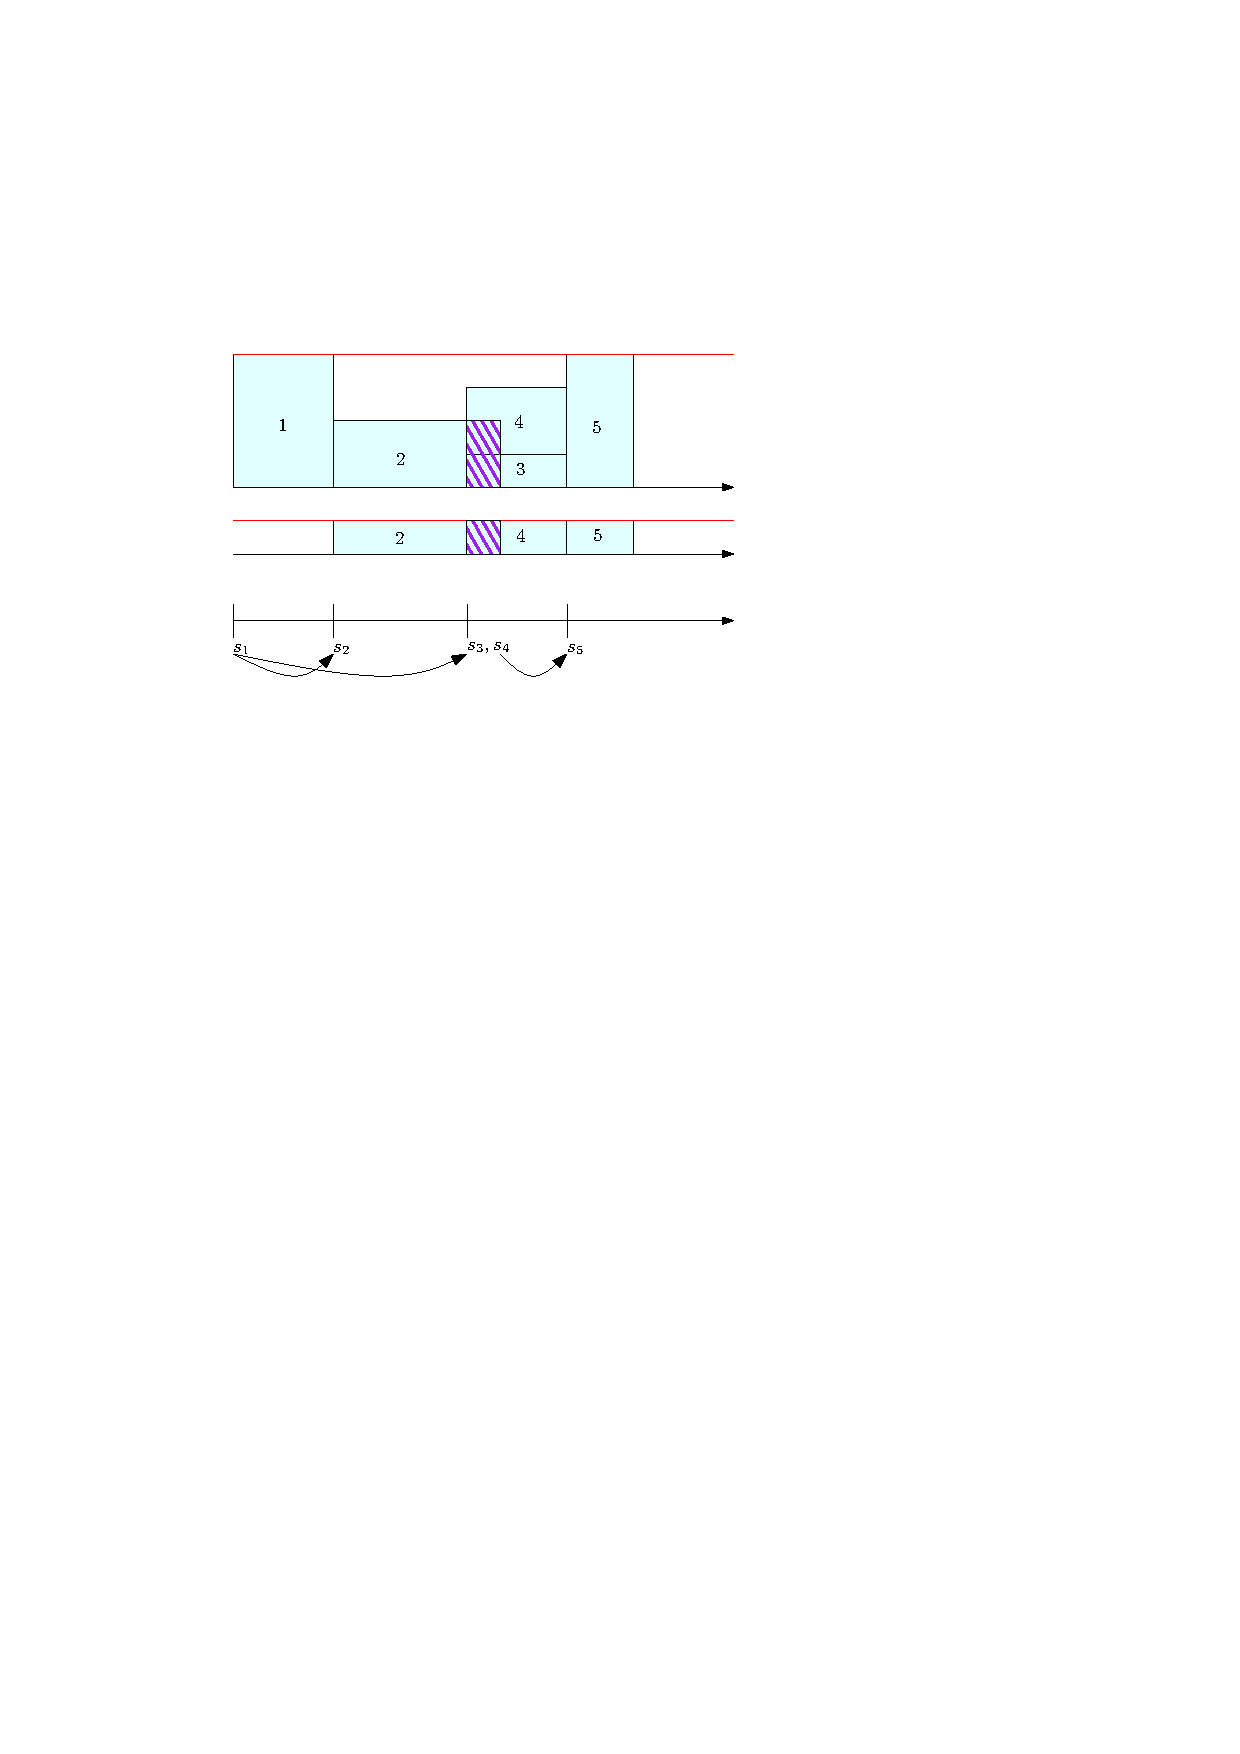
\includegraphics[width=0.7\textwidth]{fig-s1b}}
}
\end{frame}

